%% 
%% Copyright 2007-2020 Elsevier Ltd
%% 
%% This file is part of the 'Elsarticle Bundle'.
%% ---------------------------------------------
%% 
%% It may be distributed under the conditions of the LaTeX Project Public
%% License, either version 1.2 of this license or (at your option) any
%% later version.  The latest version of this license is in
%%    http://www.latex-project.org/lppl.txt
%% and version 1.2 or later is part of all distributions of LaTeX
%% version 1999/12/01 or later.
%% 
%% The list of all files belonging to the 'Elsarticle Bundle' is
%% given in the file `manifest.txt'.
%% 
%% Template article for Elsevier's document class `elsarticle'
%% with harvard style bibliographic references
\DocumentMetadata{testphase=new-or-1}
\documentclass[preprint,12pt,authoryear]{elsarticle}

% Added by V Van der Meersch
\usepackage[strings]{underscore}
\usepackage{url}
\usepackage{breakurl}
\usepackage{amsmath}
\usepackage{xcolor} % use the table option if you want color in tables
\definecolor{Accent}{HTML}{000000} 
\usepackage{hyperref}
\hypersetup{colorlinks,citecolor = Accent, linkcolor = Accent,urlcolor = Accent, breaklinks=true}
\usepackage{cleveref}
\usepackage[labelfont=normalfont]{subcaption} % useful with cleverref 
\captionsetup[subfigure]{subrefformat=simple,labelformat=simple}
\renewcommand{\thesubfigure}{\alph{subfigure}}
\usepackage{gensymb}
\usepackage{geometry}
\usepackage{pdflscape}
\usepackage{multirow} 
\usepackage{booktabs}

%% Use the option review to obtain double line spacing
%% \documentclass[authoryear,preprint,review,12pt]{elsarticle}

%% Use the options 1p,twocolumn; 3p; 3p,twocolumn; 5p; or 5p,twocolumn
%% for a journal layout:
%% \documentclass[final,1p,times,authoryear]{elsarticle}
%% \documentclass[final,1p,times,twocolumn,authoryear]{elsarticle}
%% \documentclass[final,3p,times,authoryear]{elsarticle}
%% \documentclass[final,3p,times,twocolumn,authoryear]{elsarticle}
%% \documentclass[final,5p,times,authoryear]{elsarticle}
%% \documentclass[final,5p,times,twocolumn,authoryear]{elsarticle}

%% For including figures, graphicx.sty has been loaded in
%% elsarticle.cls. If you prefer to use the old commands
%% please give \usepackage{epsfig}

%% The amssymb package provides various useful mathematical symbols
\usepackage{amssymb}
%% The amsthm package provides extended theorem environments
%% \usepackage{amsthm}

%% The lineno packages adds line numbers. Start line numbering with
%% \begin{linenumbers}, end it with \end{linenumbers}. Or switch it on
%% for the whole article with \linenumbers.
\usepackage{lineno}

\definecolor{customred}{rgb}{0.759, 0.365, 0.396}
% \definecolor{customred}{rgb}{0, 0, 0}

\journal{Ecological Modelling}

\begin{document}

\begin{frontmatter}

%% Title, authors and addresses

%% use the tnoteref command within \title for footnotes;
%% use the tnotetext command for theassociated footnote;
%% use the fnref command within \author or \affiliation for footnotes;
%% use the fntext command for theassociated footnote;
%% use the corref command within \author for corresponding author footnotes;
%% use the cortext command for theassociated footnote;
%% use the ead command for the email address,
%% and the form \ead[url] for the home page:
%% \title{Title\tnoteref{label1}}
%% \tnotetext[label1]{}
%% \author{Name\corref{cor1}\fnref{label2}}
%% \ead{email address}
%% \ead[url]{home page}
%% \fntext[label2]{}
%% \cortext[cor1]{}
%% \affiliation{organization={},
%%            addressline={}, 
%%            city={},
%%            postcode={}, 
%%            state={},
%%            country={}}
%% \fntext[label3]{}

\title{Can inverse calibration help improving process-explicit species distribution models?}

%% use optional labels to link authors explicitly to addresses:
%% \author[label1,label2]{}
%% \affiliation[label1]{organization={},
%%             addressline={},
%%             city={},
%%             postcode={},
%%             state={},
%%             country={}}
%%
%% \affiliation[label2]{organization={},
%%             addressline={},
%%             city={},
%%             postcode={},
%%             state={},
%%             country={}}

\author[inst1]{Victor Van der Meersch\corref{cor1}}\cortext[cor1]{Corresponding author: victor.vandermeersch@cefe.cnrs.fr; victor.vandermeersch@posteo.org}

\affiliation[inst1]{organization={CEFE, Univ Montpellier, CNRS, EPHE, IRD},
            city={Montpellier},
            country={France}}

\author[inst1]{Isabelle Chuine}

% \begin{abstract}
% Process-explicit models (PEMs) are expected to provide reliable projections of species range shifts because they explicitly model biological mechanisms that govern species response to climate.
% However, this kind of approach requires detailed and diverse data, which are available only for few species. 
% Inverse calibration has been identified as an avenue to help calibrating PEMs for many species---yet it is still unclear whether it can yield correctly specified parameters.
% Here, we explored the potential of such inverse calibration techniques to enhance the accuracy of PEMs. We calibrated a species distribution PEM which makes a strong focus on phenology and stress resistance using species distribution data, following two strategies: (i) calibrating all parameters simultaneously or (ii) focusing only on critical parameters. We then evaluated the realism of the parameter estimates obtained by comparing them to measurements and comparing simulated phenology to observed phenology across Europe. 
% We showed that model structure alone do not sufficiently constrain the calibration process, which may produce unrealistic parameter values. However, using inverse calibration parsimoniously can improve model performance while still allowing to simulate realistic processes.
% \end{abstract}

\begin{abstract}
\textcolor{customred}{Process-explicit models (PEMs) are expected to provide reliable projections of species range shifts because they explicitly model the biological mechanisms that drive species responses to climate.
However, their application is often limited by the need for diverse and detailed datasets, which are only available for a limited number of species. Inverse calibration has been identified as an avenue to help calibrate PEMs for many species, but it is still unclear whether it can provide biologically meaningful parameter estimates.
Here, we investigated the potential of inverse calibration techniques to improve the accuracy of PEMs. We examined the discrepancies in parameter estimates obtained by classical and inverse calibration approaches. We evaluated two inverse calibration strategies: (i) calibrating all parameters simultaneously and (ii) focusing only on critical parameters.  
We assessed the realism of the obtained parameter estimates and the simulated processes by comparing them with measurements and observations across Europe. We show that when the entire model is calibrated at once, the model structure alone may not sufficiently constrain parameter estimation, leading to unrealistic parameter values. However, selective application of the inverse calibration approach---focusing on critical parameters---can improve model performance while still simulating realistic biological mechanisms.}
\end{abstract}



%%Graphical abstract
% \begin{graphicalabstract}
% \includegraphics{grabs}
% \end{graphicalabstract}

%%Research highlights
%\begin{highlights}
%\item Inverse calibration using species distribution data can improve process-explicit model accuracy 
%\item Model structure alone does not sufficiently constrain the calibration process
%\item Careful application of inverse calibration retains realistic biological processes
%\item Inverse calibration may help using process-explicit models for many species
%\end{highlights}

\begin{keyword}
%% keywords here, in the form: keyword \sep keyword
inverse calibration \sep process-explicit model \sep process-based model \sep mechanistic model \sep species distribution \sep phenology
%% PACS codes here, in the form: \PACS code \sep code
% \PACS 0000 \sep 1111
%% MSC codes here, in the form: \MSC code \sep code
%% or \MSC[2008] code \sep code (2000 is the default)
% \MSC 0000 \sep 1111
\end{keyword}

\end{frontmatter}

\linenumbers

\clearpage
%% main text
\section{Introduction}

There have been repeated calls for focusing efforts on the development of process-explicit models (PEMs) in ecology \citep{Urban2016, Singer2016, Pilowsky2022}. Because they describe cause-to-effect relationships, they may provide more robust projections in novel climatic conditions \citep{VanderMeersch2025}. However, PEMs are still applicable to few species \citep{Evans2016}, and their widespread use would first require to address and to quantify their error and uncertainty.

We can distinguish two main source of errors in ecological models: the model's structure and the value of the parameters. The structure of a model is defined by its underlying assumptions and level of simplification. Our understanding of the regulation of the ecophysiological processes at the scale of organisms---that ultimately drive  ecosystem dynamics---has grown substantially in the last decades. This has led to significant improvements in how we represent these processes in models, e.g. plant hydraulics \citep{Ruffault2022}, although some remains challenging---such as bud dormancy \citep{Chuine2016} or carbon allocation \citep{Hartmann2020}. 
These advancements enable researchers to explore complex interacting mechanisms, providing useful insights and tools for determining conservation and management strategies in a changing world \citep{Urban2016}. However, the incorporation of new detailed processes can become a trap, as it often increases the number of poorly known parameters and limits the number of species for which these models can be applied to \citep{Franklin2020}. %parameter burden!

Process-explicit modeling depends a great deal on the calibration and the availability of \textcolor{customred}{many different data} \citep{Cabral2017}. In a classical framework, parameters are typically determined from experiments, measurements, and expert knowledge. When it is too difficult or impossible, a cost-effective solution to the problem of estimating many parameters is the use of inverse modeling to bridge observations and simulations \citep{Evans2016}. This involves adjusting the parameters until the model outputs closely match the observed data---often using an optimization algorithm with an informal objective function, or a likelihood-based statistical method \citep{Malchow2024}. Resulting parameter values are therefore conditional on the structure of the model  and the observed data: the model structure explicitly constrains how climatic factors determine species performance, and the parameters and simulation outputs depend on the observations in a similar way to statistical models \citep{Zhang2024}. Inverse modeling is increasingly used in PEMs to infer model parameters or at least some of them. Process-related data can be used to fit some part of the models separately or sequentially, e.g. tree ring series have been used to calibrate a sapwood growth submodel \citep{DeCaceres2023}, and phenological records are frequently used to calibrate phenological submodels \citep{Chuine2013}. Several data sources can also be combined to refine models \citep{Pagel2011, BenitoGarzon2019} and to calibrate several processes simultaneously in a model-data fusion fashion \citep[e.g.][]{Trotsiuk2020}. This allows to integrate data at multiple spatiotemporal scales \citep{Hartig2012, Niu2014}, and reduce potential overfitting issues \citep{Bacour2023}.

However, being able to reproduce observed data, even from several sources, does not guarantee convergence towards biologically sound parameter estimates for several reasons. First, models are a simplification of reality. They often target particular processes that are important for addressing specific questions within a specific spatiotemporal context, and some processes may be unknown or not completely understood. Whether intentional or not, this simplification may miss important processes \citep{Forrester2021}, and inverse calibration may thus lead to parameter values that compensate for these missing processes. Second, even in a structurally correct model, measurements are not likely to coincide precisely with what the model simulates \citep{Zhang2024}. Third, some parameters might also be model-specific (i.e. conceptual), and not correspond to something observable nor measurable.

Process-explicit species distribution models have rarely used inverse modeling with species distribution data available across large scales \citep{Pagel2011, Higgins2012, VanderMeersch2023}, probably because this does not align well with the general idea of this modeling approach. Traditionally, these data have only been used by correlative niche models. Yet, the large and constantly increasing volume of such data \citep{Feng2022} represents a vast amount of information that could help improve the accuracy of PEMs \citep{Evans2016}. While using only species occurrence data to infer the values of many parameters can be seen as a brute-force approach, such inverse calibrated PEMs may outperform correlative models and better reproduce the distributional patterns of the species on different spatio-temporal situations \citep{Higgins2020, VanderMeersch2025}.  Moreover, such inverse calibration could also help making PEMs easier to apply to a greater number of species and on a larger scale \citep[e.g.][]{Conradi2024}. However, a good model fit to observations, even long-term data series, does not necessarily imply a good estimation of the processes truly responsible for the observations. 
% To reach high levels of confidence in model projections,  \cite{VanderMeersch2025} showed that ecological processes should still be simulated with a high level of mechanistic realism and that using species occurrence data alone to calibrate models may not provide the highest model performance, especially in novel conditions. 

Here, we investigate the differences between parameter estimates of a PEM obtained either with a classical calibration or with inverse calibration, and what it implies in terms of realism of the simulated processes and of model performance. More precisely, we seek to understand whether and to what extent inverse calibration using species occurrence (i) can lead to realistic parameter values and processes and (ii) may help us improving PEMs. To do this, we focus on PHENOFIT, a PEM which has been used to study species range \textcolor{customred}{drivers} and to forecast species distribution shifts with past and future climate change in North America and Europe
\citep{Morin2007, Saltre2013, Saltre2015, Cheaib2012, VanderMeersch2025}. We first examine in detail 100 calibrations obtained for European beech (\emph{Fagus sylvatica} L.), and analyze the compensations between parameters and the realism of the simulated processes against observations all over Europe. We then investigate whether inverse calibration could improve parameter value estimation of some processes for which data are lacking for eight European forest tree species. 

\section{Materials and Methods}

\textcolor{customred}{All analyses were run on \textbf{\textsf{R}}. Simulation outputs, together with the code to reproduce the analysis and figures in this study, are available on GitHub at \url{https://github.com/vvandermeersch/contrast_calibrations}.}

\subsection{Process-explicit modeling with PHENOFIT}

PHENOFIT is a process-explicit model developed for temperate tree species which has been used to project their distributions using climatic conditions. It estimates the probability of presence of an adult tree \textcolor{customred}{with a proxy of the fitness} defined as the product of the probability to survive frost and drought events (survival), the proportion of flowers/fruits not killed by frost events (fruit index), and the probability that fruits reach full ripening (maturation index) at a yearly time step (\Cref{fig:phenofit}).

\begin{figure}[t]
\centering
\includegraphics[width=0.7\textwidth]{phenofit.pdf}
\caption{\textbf{Schematic description of PHENOFIT.}}
\label{fig:phenofit}
\end{figure}

Each phenological event (leaf unfolding, flowering, fruit maturation and leaf senescence) is simulated with daily climate forcing, and the model assumes that a tree species range depends mainly on the synchronization of its timing of development to the local abiotic conditions and especially the occurrence of some abiotic stresses. Thus, for example, the fitness can be reduced when a severe drought event occurs between budburst and leaf senescence, or when a substantial proportions of leaves and flowers that take part to the development of the fruits are killed by frost. In the following, we will provide a more detailed description of three important processes of PHENOFIT, which will be discussed further in this article. A precise description of the submodels and the response functions can also be found in Supplementary Material for beech.

\subsubsection{Leaf unfolding and flowering submodels}

Dates of leaf unfolding (date at which 50\% of leaves are unfold) and flowering (date at which 50\% of flowers are mature) are calculated using mechanistic phenology models \citep{Chuine2017}. Organ development is represented by a state variable, $S$, which is the integration of development rates ($R$) over time (in daily steps). The general structure of mechanistic phenology models for one specific development phase is the following:
$t_n$ such that $S_{n,t}$ = $\sum_{t=t_{n-1}}^{t_n} R_{n,t}$ = $S_n^*$ 
where $n$ is a development phase, $S_{n,t}$ is the state of development on day $t$ in phase $n$; $t_n$ is the end of phase $n$ and  $t_{n-1}$ the end of phase ${n-1}$, $R_{n,t}$ is the rate of development during phase $n$ on day $t$ which is a function of  temperature, and $S_n^*$ is the critical state required to reach $t_n$.  Several phases of development can be modeled in a single model composed of several submodels, each one describing a specific phase such as dormancy induction, endodormancy, ecodormancy, etc. In such case, phases either follow each other sequentially or can overlap depending on the development phase and the species. Leaf unfolding and flowering dates have been modelled here using 2-phases models describing both the bud endodormancy phase (bud remain dormant despite meteorological conditions that could sustain cell growth) and the ecodormancy phase (bud cell growth depends on the meteorological conditions).  Development rates ($R$) are response functions to daily temperature that can be linear or nonlinear (usually with a single optimum), \textcolor{customred}{with their functional form potentially varying across species and developmental phases. }

\subsubsection{Frost hardiness submodel}

Frost hardiness of vegetative and reproductive organs is modelled according to \citet{Leinonen1996}, as a function of the additive effect of photoperiod and temperature, and depends on the state of development (or phenological state): hardiness varies dynamically between a maximum value reached during bud winter dormancy and a minimum value reached at bud break and flowering. The model has several parameters, including the minimum level of frost hardiness ($FH_{min}$) and the maximum increase of frost hardiness ($\Delta FH_{max}$) conveyed both by photoperiod and temperature. The maximum potential level of frost hardiness is thus $FH_{min}+\Delta FH_{max}$ (see Supplementary Material for a detailed description of the model). 

\subsubsection{Fruit maturation submodel}

Fruits development is modeled with a two-phases mechanistic phenology model:  a first phase of cell multiplication and growth, and a second phase of photosynthetic assimilate accumulation. This second phase is the most important, and depends on several components including the proportion of leaves that resisted frost, water availability and photosynthetic activity. The latter varies according to temperature conditions following the unimodal function of \citet{Wang1998} which involves an optimal temperature parameter $T_{opt}$.  Fruit maturation is integrated over time at the scale of the tree crown, following a normal distribution. The mean date of fruit maturation corresponds to the date when fruit development reaches $Mat_{moy}$, and correspond to the stage 50\% of fruits are ripe,  and fruit maturation starts at $Mat_{moy}$ $-3\sigma$ and ends at $Mat_{moy}$ $+3\sigma$.

\subsubsection{Leaf senescence submodel}
Leaf senescence date (date at which 50\% of leaves have changed color or have fallen) is modelled using a 1-phase mechanistic phenology model with different response functions to temperature and to day length depending on the species \citep{Delpierre2009}. 

\subsection{Model calibration}

\subsubsection{Expert calibration}

PHENOFIT has been calibrated for several European tree species, and validated  by comparing their historical and Holocene distribution to the simulated fitness used as a proxy of species probability of presence  \citep{Saltre2013, Duputie2015, Gauzere2020, VanderMeersch2025}. Phenology submodel parameters were inferred by inverse \textcolor{customred}{calibration} using phenological \textcolor{customred}{observations} across Europe (provided through the TEMPO data portal \url{data.pheno.fr}, and the PEP725 database \url{pep725.eu}).
\textcolor{customred}{Frost hardiness submodel parameters were directly measured or found in the literature. Water stress parameters were inferred from the specific range of annual precipitation where species are found in forest inventories.}

%Finally, a few parameters are prescribed based on expert knowledge as no data to estimate them exist. 
% This expert calibration of the model does not involve species occurrence data at any point.

\subsubsection{Inverse calibration with CMA-ES algorithm and species occurrence data}

Following \citet{VanderMeersch2023}, we calibrated PHENOFIT using the covariance matrix adaptation evolution strategy (CMA-ES), which  is a robust algorithm for complex optimization problems \citep{Hansen2001}. It is inspired by Darwin's theory of evolution to find the most fit parameter sets. \textcolor{customred}{CMA-ES is easy to use, as it requires minimal tuning to effectively explore the parameter space. Global optimization algorithms such as CMA-ES are commonly used to calibrate complex models, but are not as robust as proper statistical inference (e.g., Bayesian methods) and primarily focus on identifying the most fit parameter set. To reduce computation time}, we ran the CMA-ES calibration on the multicore cluster GenOuest (\url{genouest.org}).

The objective function for the calibration was the area under the receiver operating characteristic curve (AUC), to maximize model discriminating capacity (i.e. potential to distinguish between species presences and absences). To compute the AUC, we used the same occurrence data as in \citet{VanderMeersch2023}. These were mainly extracted from the EU-Forest dataset \citep{Mauri2017}, completed with presence records extracted from the Global Biodiversity Information Facility (\url{gbif.org}) to account for tree occurrences outside forests. We removed GBIF occurrences outside natural species ranges as defined by Atlas Flora Europeae \citep{AFE2005} and EuroVegMap \citep{EVM2003}. The EU-Forest cells where the species is not reported present were considered as (pseudo-)absences. In order to reduce calibration computational costs, we selected subsets of 1000 presences and 1000 absences. Presences were sampled based on a k-means clustering to make sure that all species environmental preferences were proportionally represented (see \citet{VanderMeersch2023} for details). \textcolor{customred}{We then randomly sampled the same number of absences.}

\textcolor{customred}{First, we aimed to investigate to what extent fully calibrating the model using only species distribution data could consistently improve the model and the parameter values obtained with the expert calibration. We compared one hundred parameter sets for \emph{Fagus sylvatica}, obtained by inverse calibration on 10 different presence/absence subsets (i.e. 10 calibrations per subset),} using the same parameter bounds as in \citet{VanderMeersch2023} in order to remain in realistic parameter ranges. These calibrations are called \emph{full} inverse calibrations in the following (all parameters optimized at once, Figure S1). \\
\textcolor{customred}{Second, we wanted to determine whether inverse calibration using species distribution data could improve some parts of the model where expert calibration may fall short due to data limitations. We conducted a second set of inverse calibrations, focusing only on some model parameters, for eight different species} (\emph{Abies alba}, \emph{Betula pendula}, \emph{Fagus sylvatica}, \emph{Fraxinus excelsior}, \emph{Larix decidua}, \emph{Picea abies}, \emph{Quercus pubescens} and \emph{Quercus robur}). The parameters we calibrated corresponded to processes that we identified as responsible for false absence errors in the predictions of the expert calibration version of the model---i.e. cases where simulated fitness was low despite the species being present. To identify these processes, we calculated the relative contribution of the three sub-components of fitness: survival ($S$), fruit index ($Fr$) and maturation index ($M$) to the simulated fitness ($F$). The relative contribution of a \textcolor{customred}{sub-component} was calculated as the ratio of the product of the two other \textcolor{customred}{sub-components} over the total sum of all possible products. For example, the contribution of survival $S$ was calculated as: $\frac{Fr*M}{S*Fr+S*M+Fr*M}$. Other parameters---corresponding to processes that we did not identified as responsible for false absence errors---were fixed at the expert values. For each species, we ran 5 calibrations on 2 different occurrence subsets (i.e. 10 repetitions). These calibrations are called \emph{partial} inverse calibrations in the following. 

\subsubsection{Climate and soil data used to calibrate and run the model}

Simulations and calibrations were run with climate variables extracted from the ERA5-Land hourly dataset \citep{MunozSabater2021}, for the period 1970-2000. As in \citet{VanderMeersch2023}, we computed daily mean values of several variables: temperatures (minimum, mean and maximum), dewpoint temperature, precipitation, global radiation and wind speed. Daily potential evapotranspiration was calculated using the standard FAO Penman–Monteith equation \citep{Allen1998}. Soil water holding capacity was calculated with the field capacity and wilting point data from EU-SoilHydroGrids \citep{Toth2017} and the percentage of coarse fragments from SoilGrids250m \citep{Hengl2017}.

To assess the similarity between the different calibrations in climatic conditions that differ significantly from those used for calibration, we also ran paleosimulations, using the same climatic forcing as in \citet{VanderMeersch2025}. For this, daily data were generated with the GWGEN \textcolor{customred}{weather} generator \citep{Sommer2017}, from the monthly simulations of HadCM3B-M2.1 coupled general circulation model \citep{Armstrong2019}.

\begin{figure}
\begin{subcaptiongroup}
\phantomcaption\label{fig:1A} 
\phantomcaption\label{fig:1B}
\phantomcaption\label{fig:1C}
\phantomcaption\label{fig:1D}
\phantomcaption\label{fig:1E}
\phantomcaption\label{fig:1F}
\end{subcaptiongroup}
\centerline{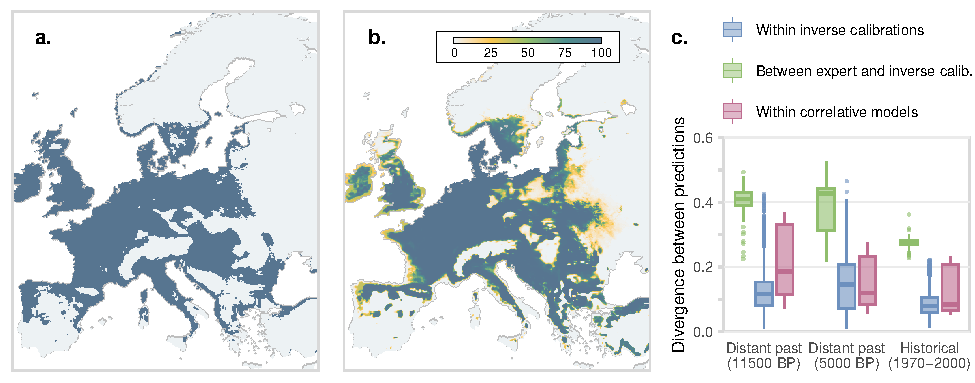
\includegraphics{fig1-1.pdf}}
\caption{Simulated potential presence of \emph{F. sylvatica} with \textbf{(a,c)} the expert parametrization and \textbf{(b,d)} the set of 100 \emph{full} inverse calibrations, in the historical climatic conditions \textbf{(a,b)} and in the paleoclimatic conditions \textbf{(c,d)}. Simulated fitness is converted to presence/absence (blue/grey) using the optimal threshold that maximizes the true skill statistic (TSS). 
\textcolor{customred}{\textbf{(e)} Observed distribution of \emph{F. sylvatica}, with both continuous area of occupancy and isolated populations, based on data gathered by \citet{Caudullo2017}.}
\textbf{(f)} S\o rensen dissimilarity between inverse calibrations, and between expert calibration and inverse calibrations. S\o rensen dissimilarity between 5 different correlative species distribution models (from \citealp{VanderMeersch2025}) is shown for comparison. BP stand for "Before Present" (i.e. 1950).}
\label{fig:1}
\end{figure}

\subsection{Parameter estimates' evaluation}

We partitioned the 100 \emph{full} inverse calibrations of \emph{Fagus sylvatica} using two k-means clustering procedures in a row (\Cref{fig:2A}). The first clustering was based on the simulated leaf dormancy break and leafout dates. Then, within each cluster, the second clustering was computed based on the fruit maturation and leaf senescence dates.

In order to verify that the parameter values after calibration lead to realistic processes, we calculated root-mean-square errors (RMSE) between simulated phenological dates and observed dates. The latter were extracted from two databases, PEP725 and TEMPO, covering the period 1970-2000, essentially in Central Europe (Figure S2). For \emph{Fagus sylvatica}, we used 59484 observations of leafout, 10449 of flowering, 23606 of fruit maturation and 71469 of leaf senescence (\Cref{fig:3}). Moreover, we used 16329 obs. of \emph{Betula pendula} flowering, 21813 obs. of \emph{Picea abies} flowering and 49236 of \emph{Quercus robur} fruit maturation (\Cref{fig:5}).


\section{Results}

\subsection{Coherent and stable predictions despite process discrepancies}

The similarity between the simulated ranges of European beech obtained with the 100 \emph{full} inverse calibrations was relatively stable over the last 12k years. The disagreements were mostly at the margins of the distribution (\Cref{fig:1B,,fig:1D}). The S\o rensen dissimilarity between the inverse calibration projections was lower in historical conditions (median = 0.0805 [IQR = 0.0605 - 0.106]) than in the distant past, e.g. 11500 years ago (0.116 [0.0813 - 0.154], \Cref{fig:1F}). However it increased relatively little while moving back to the past, i.e. to more dissimilar climatic conditions, compared to the dissimilarity between expert calibration and inverse calibrations, from 0.276 [0.268 - 0.283] in the present to 0.410 [0.391 - 0.429] at 11500 BP.

The relatively similar projections of the 100 \emph{full} inverse calibrations, however, resulted from simulated biological processes that differed substantially (\Cref{fig:2}). Regarding bud development, 65 calibrations (clusters blue and green, \Cref{fig:2A})  had a short endodormancy phase (ending in November or December of the previous year, \Cref{fig:2B}) and a longer ecodormancy phase (with an average duration of 187 days $\pm$ 56.9). On the contrary, the remainder of the 34 calibrations (clusters yellow and orange, \Cref{fig:2A}) had a longer endodormancy phase (ending in February or March) and a shorter ecodormancy phase (with an average duration of 89.4 days $\pm$ 38.7). Note that one of the calibrations stood out due to both short endodormancy and short ecodormancy (\Cref{fig:2B,,fig:2C}). Similarly, two behaviors can be identified in terms of fruit maturation: 83 calibrations (clusters green and yellow) led to early maturation (August/September, \Cref{fig:2D}), and 16 led to late maturation (October/November, \Cref{fig:2D}).

\begin{figure}[hb]
\begin{subcaptiongroup}
\phantomcaption\label{fig:2A} 
\phantomcaption\label{fig:2B}
\phantomcaption\label{fig:2C}
\phantomcaption\label{fig:2D}
\phantomcaption\label{fig:2E}
\end{subcaptiongroup}
\centerline{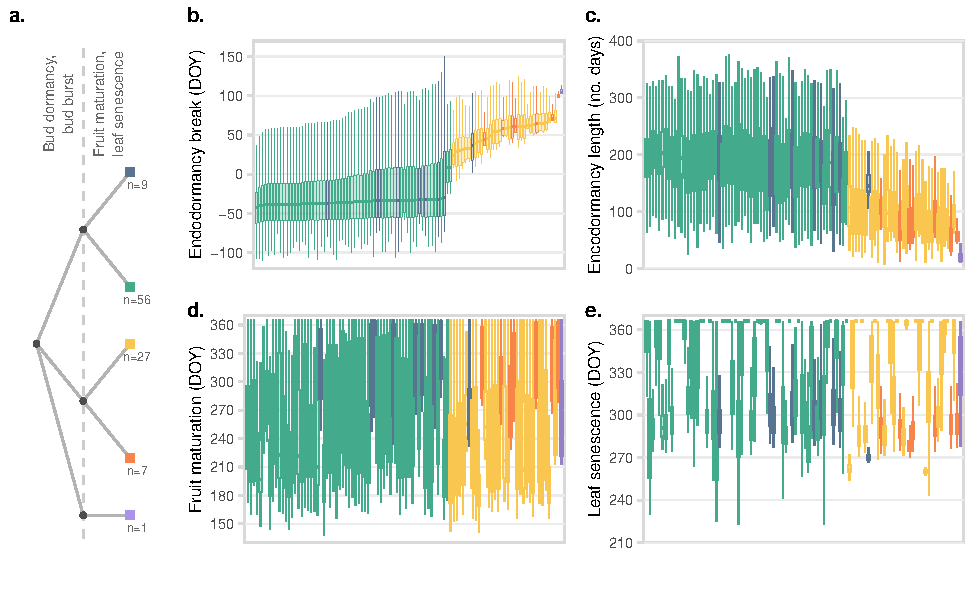
\includegraphics{fig2-1.pdf}}
\caption{\textbf{(a)} Partition of the 100 \emph{full} inverse calibrations for \emph{Fagus sylvatica} after a two-step clustering. First clustering was based on the simulated leaf dormancy break and leafout dates. Second clustering was computed based on the fruit maturation and leaf senescence dates. \textbf{(b,c,d,e)} Simulated dates (day of the year, DOY) of \textbf{(b)} bud endodormancy, \textbf{(c)} bud ecodormancy, \textbf{(d)} fruit maturation and \textbf{(e)} leaf senescence. Colors correspond to the different clusters in \textbf{(a)}. Note that we do not show flowering as it occurs almost simultaneously with leaf unfolding.}
\label{fig:2}
\end{figure}

\subsection{Errors in the simulated processes}

These strong discrepancies between simulated processes inevitably led to differences in terms of agreement with phenological observations across Europe (\Cref{fig:3}). The first group of calibrations (short endodormancy/long ecodormancy) had a median error of 28.3 days for the budburst date, and up to 120 days for the worst calibration. The second group (long endodormancy/short ecodormancy) had a smaller median error of 16.3 days [7.73 - 27.4]. \textcolor{customred}{Both tend to overestimate the leafout day (with an average bias of 24.0$\pm$25.9 days), and} performed worse than the expert version of the model (6.95 days [3.36 - 12.1], \Cref{fig:3A}) whose parameters were calibrated using some of the phenological observations. Regarding fruit maturation, the late-maturation cluster (blue and orange) got a median error of 17 days [8 - 29], closer to the expert version (13 days [6 - 24]). Moreover, inverse calibrations showed almost no year where fruit maturation could not occur unlike the expert version, whose parameters did not allow for ripe fruits in more than 50\% of the cases (\Cref{fig:3C}). For leaf senescence, contrary to the expert version which always predicted a senescence date, 43\% of the calibrations led to no senescence date for at least 50\% of the cases (\Cref{fig:3D}), and 34\% to no senescence at all. These calibrations belonged exclusively to the early-maturation cluster (green and yellow), whereas the late-maturation cluster got a median error of senescence date of 14.6 days [8.75 - 22], slightly higher than the expert version (10.8 days [6 - 16]). \textcolor{customred}{On average, inverse calibrated models tend to overestimate the senescence date, with a bias of 16.9$\pm$25.9 days.}

\begin{figure}
\centering
\begin{subcaptiongroup}
\phantomcaption\label{fig:3A} 
\phantomcaption\label{fig:3B}
\phantomcaption\label{fig:3C}
\phantomcaption\label{fig:3D}
\phantomcaption\label{fig:3E}
\end{subcaptiongroup}
\centerline{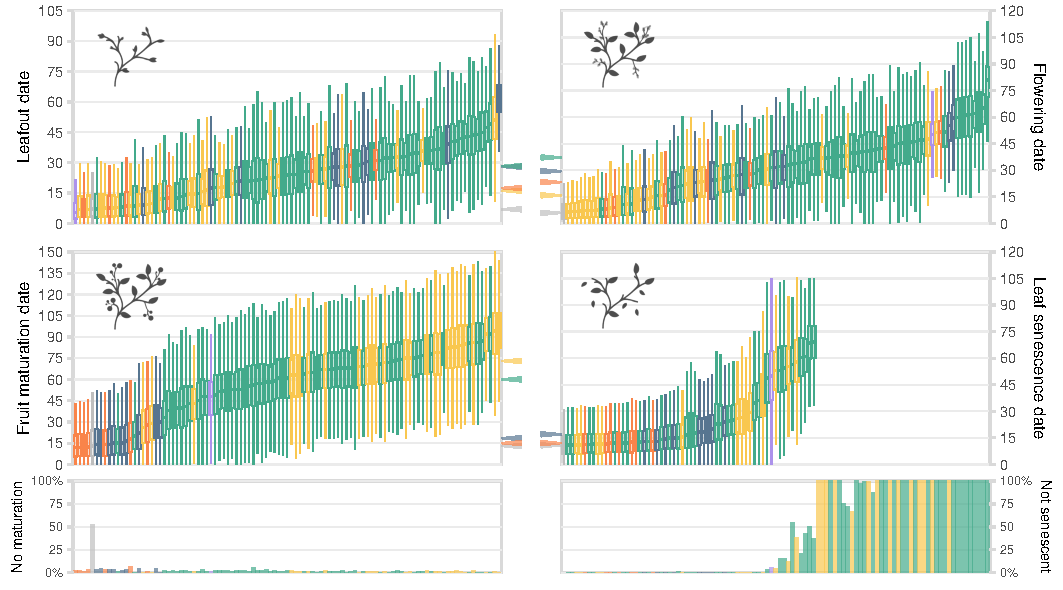
\includegraphics{fig4-1.pdf}}
\caption{Root-mean-square error (RMSE) between phenological dates that were observed for \emph{Fagus sylvatica} between 1970 and 2000 and those that were predicted by the 100 \emph{full} inverse calibrations, for \textbf{(a)} leaf unfolding, \textbf{(b)} flowering, \textbf{(c)} fruit maturation and \textbf{(d)} leaf senescence. For fruit maturation and leaf senescence, the lower panels show the percentage of cases (year x site) for which the parameter sets predict that the event does not occur (i.e. no maturation or no leaf senescence). Colors are based on the clustering shown in Fig. 2, grey corresponds to the expert parameter set. Arrows in the middle indicate the median RMSE for each group.}
\label{fig:3}
\end{figure}

\subsection{Partial calibrations on selected parameters}

The previous results showed significant differences between the calibrations in terms of simulated processes and of agreements with the available observations. However, some of the calibrations simulated processes that were relatively consistent with observations, and this was confirmed in the following when attempting to inversely calibrate the processes causing false absence errors with the expert version of the model. Most partial calibrations resulted in an AUC higher than 0.8 (\Cref{fig:4}), and in the best-case scenario an increase of more than 0.4 for spruce \emph{(Picea abies}), where we transitioned from a model worst than random to one with a good discriminatory ability.

The lack of data, particularly for fruit maturation, prevented us from checking the realism of partial calibrations for all species. We were able to evaluate the inverse calibrations of the fruit maturation date submodel for beech (\emph{Fagus sylvatica}) and pedunculate oak (\emph{Quercus robur}) (\Cref{fig:5A}), of the flowering date submodels for birch (\emph{Betula pendula}) and spruce  (\emph{Picea abies}) (\Cref{fig:5B}), and the frost hardiness submodel for fir ({\emph{Abies alba}), beech and birch (\Cref{fig:5C}). For beech, most calibrated parameter sets converged towards a median error of the fruit maturation date ranging from 11 to 16 days (except one with a median error of 24 days), close to the expert version error of 13 days (\Cref{fig:5A}). Similarly to the full calibrations, they also corrected the non-fruit maturation issue of the expert version. For pedunculate oak , half of the calibrations led to errors in the fruit maturation date similar to the expert version, around 16 days, and only 9.67 days [4.33 - 17] for the best parameter set (\Cref{fig:5A}). Regarding the flowering date of birch, 2 out of 10 partial calibrations resulted in a lower median error (5.91 days [2.55 - 11.6] and 5.91 days [2.72 - 11.4]) than the expert parameter set (8.87 days [4.21 - 14.9]). However, some had a much higher median error, up to 50.2 days (\Cref{fig:5B}). For spruce, the best calibration in terms of RMSE simulated no flowering in 37.3\% of the cases. Apart from this one, the other 9 calibrations had a higher median error (between 18.3 days [10.3 - 27.9] and 29.7 days [20.0 - 41.7]) than the expert version of the model (11.5 [5.68 - 18.9]). Finally, the frost resistance submodel parameter estimates were very close to the expert version value in only one third of the cases (\Cref{fig:5C}).

\begin{figure}[hb]
\centering
\centerline{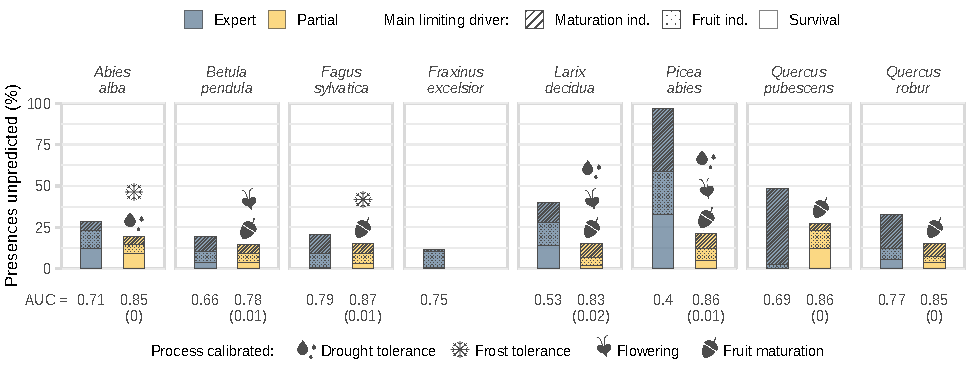
\includegraphics{fig6-1 - icons.pdf}}
\caption{Results of the \emph{partial} calibrations for the eight species considered, where only some of the parameters were optimized (pictograms indicate which processes have been recalibrated using species distribution data). The y-axis shows the percentage of observed presences that are predicted as absences by the model (i.e. \emph{false absences}), and the bar patterns represent the main simulated processes explaining these errors. The bottom row shows the average AUC (a classic discrimination performance metric) and its standard deviation in parenthesis.}
\label{fig:4}
\end{figure}

\section{Discussion}

Our results show that inverse calibration of process-explicit models (PEMs) using species distribution data does not necessarily lead to realistic parameters and simulated processes. They further demonstrate that inverse calibration can be highly useful as a model diagnostic tool, and, more importantly, to calibrate selected parts of a model where specific data and expert knowledge are lacking, albeit important cautions.

\subsection{Inverse calibration can lead to accurate species range predictions despite unrealistic parameter estimates}

% Some parameter sets outperformed the expert calibrations used for this study (especially when few data are available for the expert calibration) when predicting species distributions, but most resulted in larger errors when predicting the dates of the phenological events---up to 2 months in the worst case (\Cref{fig:3}).
When calibrating the entire model, few parameter sets outperformed the expert calibrations used for this study (especially when few data are available for the expert calibration), but most resulted in larger errors when predicting the dates of the phenological events---up to 2 months in the worst case (\Cref{fig:3}).
For some other processes, inverse calibration induced even unrealistic functional traits. For example, a large portion of the calibrations considered beech as an evergreen species, or at least not senescent, in some regions (\Cref{fig:3D}).

Despite similar predictions of species distribution (\Cref{fig:1B}), we observed that simulated processes could strongly diverge between calibrated models. Some calibrated models led for example to a short endodormancy phase, followed by a longer ecodormancy phase, and \textit{vice-versa} (\Cref{fig:2A,,fig:2B}). This arises because the compensation between these two processes has little effect on the functional trait they regulate, the leaf unfolding date, and thus on the predicted distributions. The non-identifiability of parameter values obtained with \textcolor{customred}{our inverse calibration framework}---i.e. when different sets of parameters may result in equivalent model outputs, also called equifinality---is a known issue \citep{He2017, Cameron2022, VanderMeersch2023, Malchow2024}. Here we show that compensations can occur between components of a same process or between different processes. For example, errors between simulated and observed leafout dates vary greatly across calibrated models (\Cref{fig:3A}), suggesting that these errors are compensated by another process---for example, leaf frost hardiness or fruit development. 

Unexpectedly, these discrepancies in the simulated individual processes did not cause a sharp increase in the dissimilarity between the predictions of the different calibrated models over the Holocene (\Cref{fig:1C,,fig:1D,,fig:1F}), even in the very different climatic conditions of the Early Holocene (Figure S3). In other words, while inverse calibration led sometimes to very different parameter sets and thus very different "phenotypes" (early/late budburst, deciduous/evergreen...), the predictions nevertheless remained consistent across long time scales and novel climatic conditions. Therefore, the optimization algorithm \textcolor{customred}{CMA-ES} manages to consistently find  a similar relationship between climatic conditions and the higher-level model output (fitness), regardless of the divergent lower-level processes (frost hardiness, fruit development, etc.). The link between climate and species distribution as captured in the occurrence data thus seems to constrain the model's behavior without necessarily capturing the realistic underlying processes. In other words, the optimization algorithm appears to accommodate the model structure, making it flexible enough to fit the data well. However, this strength of the optimization algorithm is also its weakness: the model structure and the mathematical functions used to describe the processes are not sufficient to constrain the parameter estimates. Thus, contrarily to what is usually assumed \citep{Higgins2020}, here we find that PEMs are not necessarily less flexible than correlative models because of their structure. This highlights the importance of not focusing solely on some metrics of (apparent) performance, even in novel climatic conditions, but rather investigating the intermediate outputs of the model. \textcolor{customred}{This is crucial to ensure that process-explicit models keep their biological meaning, which is one of their key advantages over more flexible methods that lack mechanistic understanding.}

Finally, and similarly to correlative models \citep{BarbetMassin2010, Duputie2014},  PEMs are affected by the bias in the occurrence data used for the calibration. For example, all simulations predict a low fitness of \emph{Fagus sylvatica} in south-western France contrary to the expert model predictions (\Cref{fig:1B}), whereas its absence is potentially more attributable to the legacy of forest management (vast maritime pine plantations) than to truly limiting climatic conditions as the presence of some old relict beech forests in the region suggests \citep{Lafontaine2014}. \textcolor{customred}{Similar legacies of forest management exist for silver fir (\emph{Abies alba}), whose climatic niche appears broader than its realized distribution \citep{Tinner2013}, and for spruce (\emph{Picea abies}),  which is a commercially very important species.}

\begin{figure}
\centering
\begin{subcaptiongroup}
\phantomcaption\label{fig:5A} 
\phantomcaption\label{fig:5B}
\phantomcaption\label{fig:5C}
\end{subcaptiongroup}
\vspace*{-1cm}
\centerline{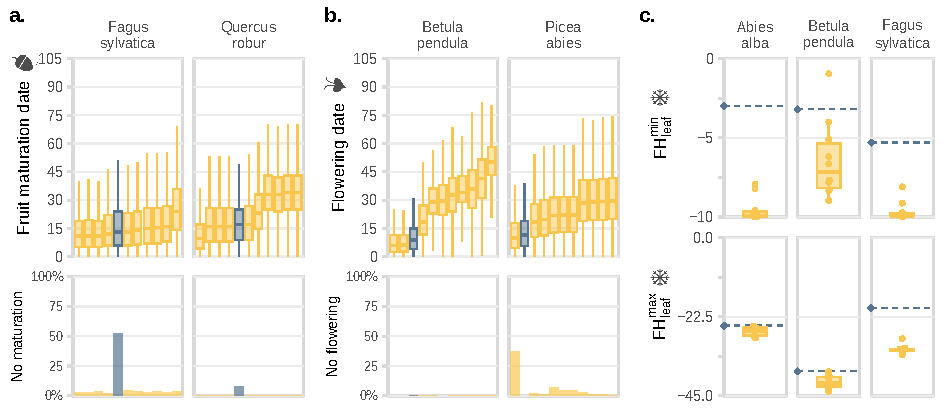
\includegraphics{fig7-1 - icons.pdf}}
\caption{Root-mean-square error (RMSE) between phenological dates that were observed for the different species between 1970 and 2000 in Europe and those that were predicted by the partial calibrations (yellow) and the expert calibration (blue), for \textbf{(a)} fruit maturation and \textbf{(b)} flowering. \textbf{(c)} Distribution of the frost hardiness parameter estimates after partial calibration. The blue dotted line shows the value in the expert version of the model.}
\label{fig:5}
\end{figure}


\subsection{Inverse calibration can help identifying model limitations and opportunities for improvement}

Our results reveal both the power and the shortcomings of inverse calibration \textcolor{customred}{using species occurrence data} in ecological modeling, and call for a careful use of the method when one aims at providing projections in very different conditions from the calibration conditions. They further suggest that inverse calibration can be an effective diagnostic tool to improve PEMs, both in terms of model hypotheses and parametrization. Using occurrence data to calibrate such models might be fruitful, if a detailed evaluation of the realism of the parameter estimates and the values of the functional traits (phenotypes) they produce is carried out\textcolor{customred}{---and if the data used is correct.}

Inverse calibration can help identify processes that are not accounted for, or incompletely accounted for in the model, even though they may be important in the context of the study.  Reversely, inverse calibration can help identify processes taken into account in the model which have little impacts on the targeted outputs. For example, the discrepancies between leaf senescence date predictions across the different calibrations (\Cref{fig:2D,,fig:3D}) highlight that, in the model, leaf senescence date is more weakly constrained during the calibration compared to other traits because it has more limited impact on fitness \textcolor{customred}{in the PHENOFIT model}. More precisely, the senescence date affects fitness if it occurs before the end of fruit development but late senescence date does not affect fitness because there is no nutrient remobilization in the model that would confer an advantage in loosing leaves before the first frost event. In this example inverse calibrations indicate that it might be opportune to refine the model by adding nutrient remobilization.

Using inverse calibration with species occurrence data can further improve PEMs in several ways. First, it can help improving the modeling of processes that have a significant impact on the model outputs but for which we have limited measurements and observations. For example, for forest tree species, observations of fruit maturation are often sparse and limited to some areas. It is therefore difficult to find the correct parameter values for the fruit maturation submodel, which can cause errors (e.g. beech, \Cref{fig:3C}). Relaxing the fruit maturation submodel parameters in the expert version of the model for several species, and calibrating them using inverse calibration and species occurrence data (\Cref{fig:4}), not only increased the model goodness-of-fit (i.e AUC)---as expected---but also resulted in more accurate predictions of fruit maturation dates on average (\Cref{fig:5A}).

Second, as pointed by \cite{Harrison2021}, the estimation of PEM parameters are sometimes \emph{ad hoc} or rely on outdated data. Thus \emph{partial} inverse calibration can also be an opportunity to identify the parameters where the disagreement between the expert value and the calibrated values is systematically significant. For example, the maximum frost resistance of beech buds during winter ($FH_{min}+\Delta FH_{max}$) is $-25.3$\degree C in the expert version of the model, while inverse calibration yields an average value of $-41.4$\degree C (\Cref{fig:5C}), which is notably lower and suggests the need to reassess the expert value. Recent studies indeed indicate values closer to $-32$ to $-37$\degree C \citep{Delaporte2015, Kreyling2014, Lenz2016, Baffoin2021, CharraVaskou2012}.
 
However, we should keep in mind that the parameter values inferred with such \emph{partial} calibrations are conditioned by the rest of the fixed processes and by the structural errors and hypotheses of the model. For example, the minimum frost resistance of leaves at leaf unfolding, ${FH}^{min}$, converged towards an unrealistically low value of -10°C for both beech and fir (the lower bound constraining the optimization of this parameter, \Cref{fig:5C}). The parameters of the leaf unfolding submodel might actually be not valid for the entire study area (e.g. existence of local adaptation of populations to climatic conditions; \citealp{Kreyling2014, Lazic2024}) and the calibration algorithm may have compensated for too early leaf unfolding dates with a higher frost resistance of leaves. Local adaptation could explain some variation in parameter values between expert and inversely calibrated versions of the model, but likely not of this magnitude. More probably, this difference points to a weakness in the model, which does not account for possible different resistance to frost between a freshly unfold leaf and a mature leaf, which may have biased the estimation of ${FH}^{min}$. Parameter estimates obtained by inverse calibration using species distributions might thus also pinpoint potential improvement of the models.

\subsection{Inverse calibration can provide a more comprehensive assessment of model uncertainties}

In many applications of PEMs, parameter uncertainties are not considered and simulations are run with a single parameter sets \citep{Niu2014, Lobell2010}. Typically, in previous studies using PHENOFIT, all parameters had a chosen fixed value, and model deterministic outputs did not account for parameter uncertainties. To avoid being overconfident with individual model projections, multiple inverse calibrations could be used to generate an ensemble of model projections (\Cref{fig:1B}). The spread of model outputs across the ensemble may then allow to assess the uncertainty associated with the parameter values \citep{Simmonds2024}, and to provide a more comprehensive range of projections rather than single deterministic outcomes.

However, these projections will always be contingent on model hypotheses and structure. The representation of processes in models may indeed represent a large source of uncertainty, as processes can usually be modeled with various equations determining their functional form \citep{Keenan2011}. One could test a set of alternative mathematical structure to quantify the impacts of this structural uncertainty \citep{Huber2020}. An efficient way could be to include them during the calibration procedure, i.e. by also optimizing similarly plausible process formulations rather than just the parameter values, or by using highly flexible functions where the parameter values determine the function type \citep{Chuine2000}.

Overall, inverse calibration using species distribution data show promise as a method to enhance specific model components in the absence of more precise data. However, process-explicit model structure and mathematical functions alone do not sufficiently constrain the calibration process. To avoid producing unrealistic parameter estimates, inverse calibration thus necessitates a careful application and a thorough evaluation to ensure realistic modeling outcomes. 

A more robust application of inverse modeling would involve integrating diverse types of data simultaneously, in a multi-objective fashion, to leverage complementary information from various sources \citep{Cameron2022}. \textcolor{customred}{It would also require inference methods that can accomodate unbalanced data streams along with model structural assumptions \citep{Oberpriller2021}}. In the near future, the increasing availability of high-resolution data---such as remote sensing and LiDAR---combined with an effective inverse-calibration framework will probably enable a better integration of large-scale data and ultimately a more accurate model parametrization\textcolor{customred}{---along with a thorough propagation of parameter uncertainty.} This could even pave the way for real-time continuous data integration and model recalibration, transforming ecological models into digital twins \citep{Koning2023}.

\section*{Acknowledgments}
\noindent We would like to thank the GenOuest computing cluster team for their technical support and for providing the computational resources required for this study. Victor Van der Meersch was supported by a GAIA doctoral school PhD Fellowship.

\section*{Data availability}
\noindent Simulation outputs, together with the code to reproduce the analysis and figures in this study, are available on GitHub at \url{https://github.com/vvandermeersch/contrast_calibrations}.

%% The Appendices part is started with the command \appendix;
%% appendix sections are then done as normal sections

\clearpage
\appendix

% \section{PHENOFIT processes and parameters}
% \label{sec:sample:appendix}

\newgeometry{left=1in,right=0in,top=0in,bottom=0.5in,nohead}
\begin{landscape}
\input{tablePHENOFIT}
\end{landscape}
\restoregeometry

\newpage

\section{Leinonen frost hardiness model}

The model developed by \cite{Leinonen1996} predicts the frost hardiness of tree buds, i.e. their ability to withstand frost, and frost damages. The model uses daily temperature, photoperiod, and bud development state (phenological state) as the drivers of bud hardening and dehardening. In particular, a tree frost hardiness undergoes acclimation in response to two factors : decreasing temperatures and shorter days. The damage caused by freezing thus depends on the minimum temperature of day $t$ and the actual frost hardiness $FH_t$ reach on day $t$:
\begin{equation}
FH_t = FH_{min} + CR_t * (\Delta FHT_t + \Delta FHP_t)
\end{equation}

\noindent $FH_{min}$ is the minimum level of frost hardening of a bud expressed in degree celsius and it corresponds to the level after bud break when leaves have just unfold (see table above), $CR_t$ is the hardening competence (which depends on the phenological state provided by the phenology model), $\Delta FHT_t$ is the increase of frost hardiness induced by temperature and $\Delta FHP_t$ is the increase of frost hardiness induced by photoperiod.

\paragraph{Exposure to cold temperatures}

The temperature component $\Delta FHT_t$ is modelled by a piece-wise linear function depending on the daily minimum temperature $T_t$:

\begin{equation}
  \Delta FHT_t =
    \begin{cases}
      \Delta FHT_{max} & \text{if $T_t < Te_2$}\\
      \Delta FHT_{max}*(1-\frac{T_t-Te_2}{Te_1-Te_2}) & \text{if $Te_2 \leq T_t \leq Te_1$}\\
      0 & \text{if $T_t > Te_1$}
    \end{cases}       
\end{equation}

\noindent $\Delta FHT_{max}$, $Te_2$, and $Te_1$ are described in the table above. $\Delta FHT_{max}$ correspond to the maximum level of increase in frost hardiness that temperature can induce when the bud is fully dormant during winter.

\paragraph{Photoperiod sensitivity}

The photoperiod component $\Delta FHP_t$ is modelled by a piece-wise linear function depending on the daily night length $NL_t$:

\begin{equation}
  \Delta FHP_t =
    \begin{cases}
      \Delta FHP_{max} & \text{if $NL_t > NL_2$}\\
      \Delta FHP_{max}*\frac{NL_t-NL_1}{NL_2-NL_1} & \text{if $NL_1 \leq NL_t \leq NL_2$}\\
      0 & \text{if $NL_t < NL_1$}
    \end{cases}       
\end{equation}

\noindent $\Delta FHP_{max}$, $NL_2$, and $NL_1$ are described in the table above. $\Delta FHP_{max}$ correspond to the maximum level of increase in frost hardiness that photoperiod can induce when the bud is fully dormant during winter. $FH_{min} + \Delta FHT_{max}$ + $\Delta FHP_{max}$ corresponds to the maximum level of frost hardiness that the bud can reach when it is fully dormant during winter. 

\newpage

\newgeometry{right=0.5in,top=0.2in,bottom=1in,nohead}
\section{Fitted parameter values for \emph{Fagus sylvatica}}

\begin{figure}[hp]
\vspace*{-0.5cm}
\hspace*{-0.5cm}
\centerline{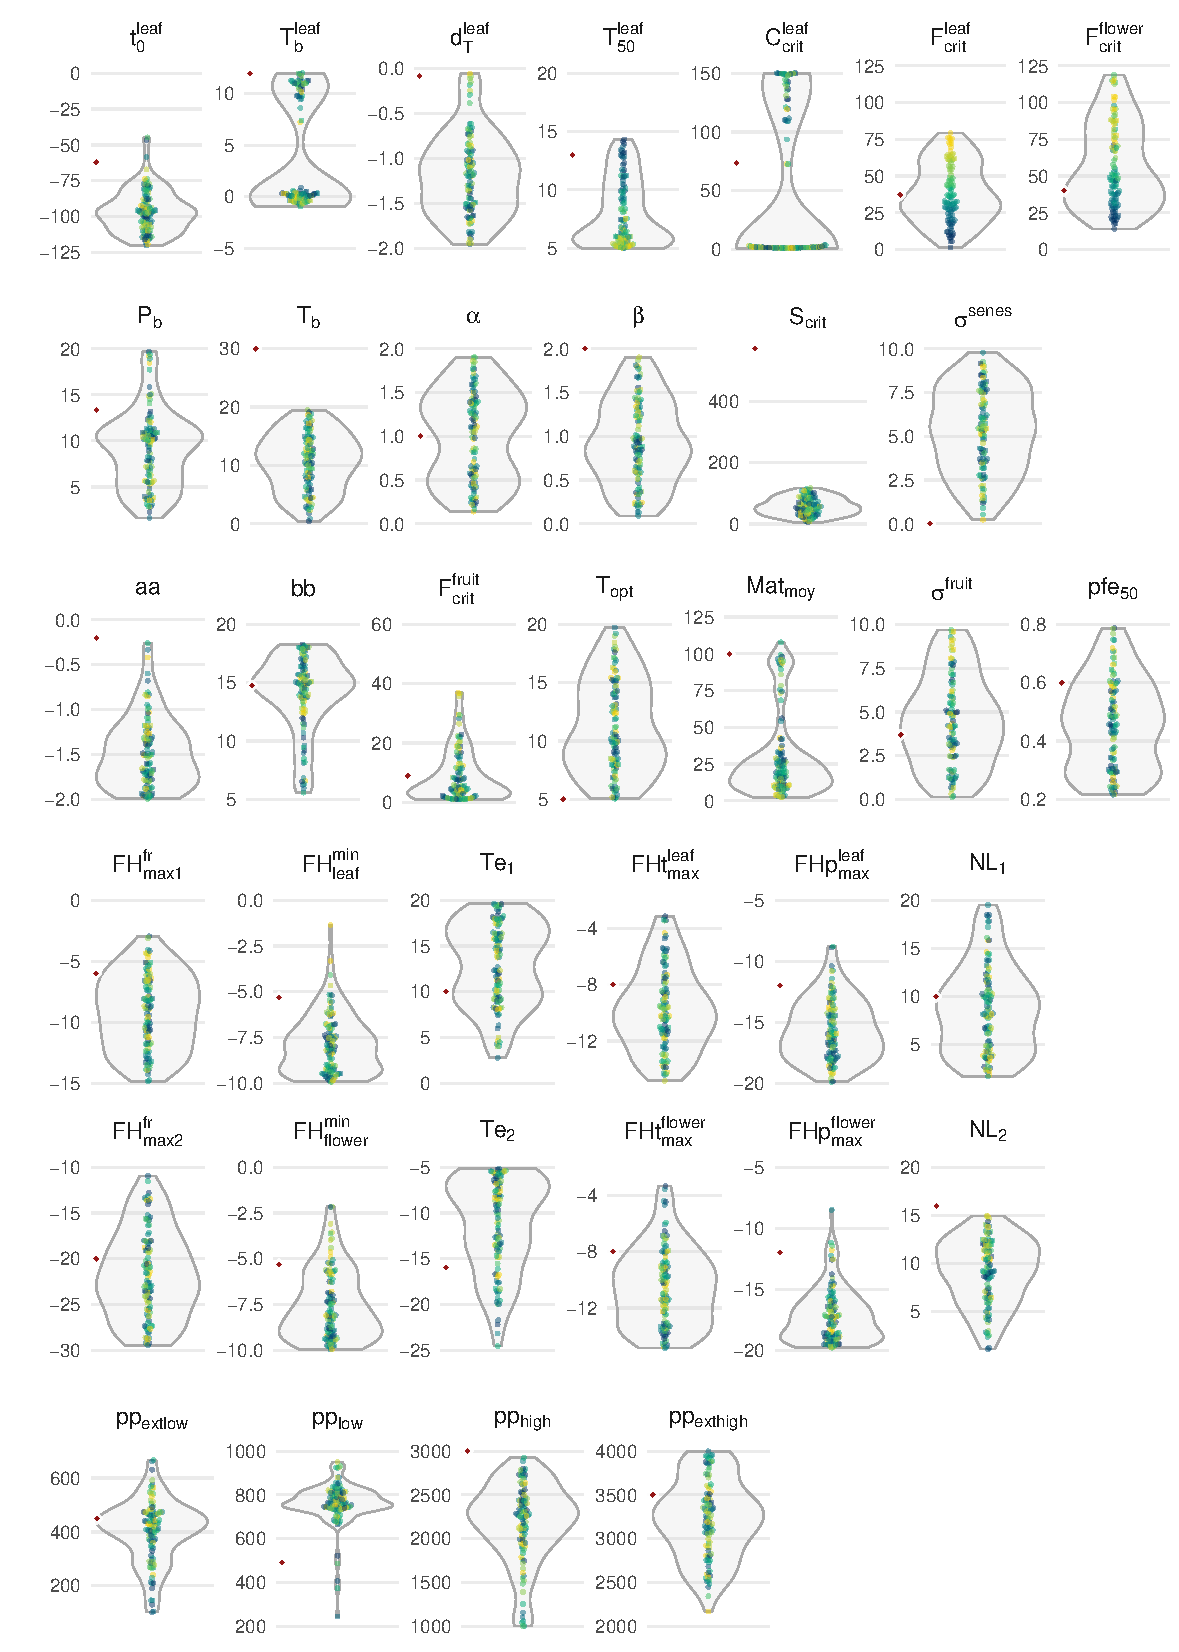
\includegraphics[width=0.95\textwidth]{parameters_fsylvatica.pdf}}
\caption{\textbf{CMA-ES calibration of PHENOFIT parameters for \emph{Fagus sylvatica}.} One panel per parameter. Y-axis limits are lower and upper bounds used during calibration. Each point is a calibrated parameter value and colour gradient represents the values of parameter $F_{crit}^{leaf}$ . Red diamonds are parameter values used in the expert version of the model.}
\vspace*{-10cm}
\end{figure}


\newpage

\section{Phenological records in Europe}

\begin{figure}[hp]
\centering
\centerline{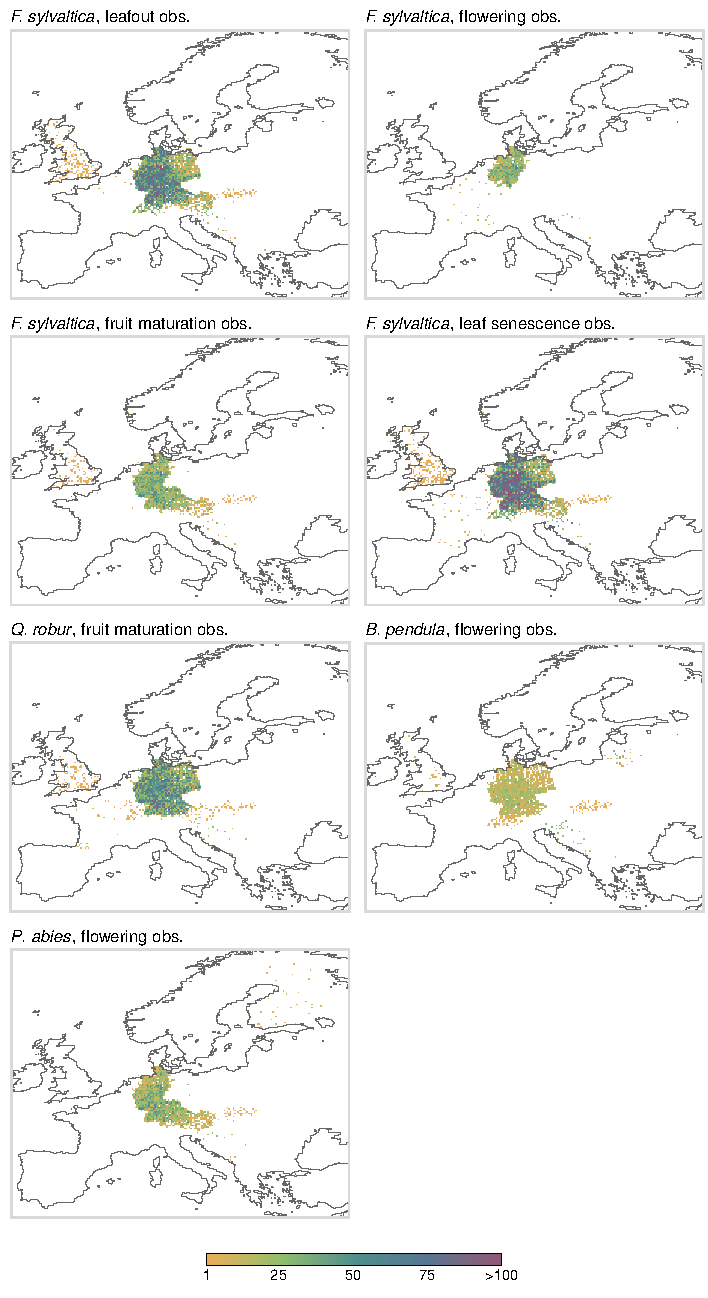
\includegraphics[width=0.7\textwidth]{figS1-1.pdf}}
\caption{\textbf{Observations used to calculate RMSE on simulated phenological dates.} These observations were extracted from the PEP725 (\url{pep725.eu}) and the TEMPO (\url{data.pheno.fr}) databases, for the period 1970-2000. Note that they were aggregated to 0.2\degree~spatial resolution, to enhance the readability of the figure.}
\vspace*{-10cm}
\end{figure}
\restoregeometry

\clearpage

\section{Climatic dissimilarity over the Holocene}

\begin{figure}[htpb]
\centering
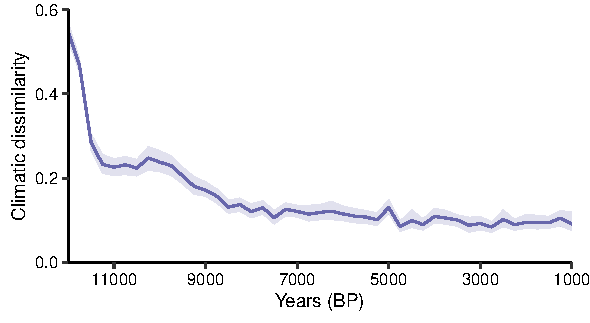
\includegraphics{figS2-1.pdf}
\caption{\textbf{Climatic dissimilarity between past conditions and historical conditions.} The metric was calculated as the Sørensen dissimilarity between climatic hypervolumes (a metric of overlap in multidimensional space). See \cite{VanderMeersch2025} for details.}
\end{figure}

\newpage


%% If you have bibdatabase file and want bibtex to generate the
%% bibitems, please use
%%

\bibliographystyle{elsarticle-harv} 
\bibliography{contrast}

%% else use the following coding to input the bibitems directly in the
%% TeX file.

% \begin{thebibliography}{00}

% %% \bibitem[Author(year)]{label}
% %% Text of bibliographic item

% \bibitem[ ()]{}

% \end{thebibliography}
\end{document}

\endinput
%%
%% End of file `elsarticle-template-harv.tex'.
